% !Rnw weave = knitr
\documentclass[a4paper, french, 11 pt]{article}\usepackage[]{graphicx}\usepackage[]{xcolor}
% maxwidth is the original width if it is less than linewidth
% otherwise use linewidth (to make sure the graphics do not exceed the margin)
\makeatletter
\def\maxwidth{ %
  \ifdim\Gin@nat@width>\linewidth
    \linewidth
  \else
    \Gin@nat@width
  \fi
}
\makeatother

\definecolor{fgcolor}{rgb}{0.345, 0.345, 0.345}
\newcommand{\hlnum}[1]{\textcolor[rgb]{0.686,0.059,0.569}{#1}}%
\newcommand{\hlstr}[1]{\textcolor[rgb]{0.192,0.494,0.8}{#1}}%
\newcommand{\hlcom}[1]{\textcolor[rgb]{0.678,0.584,0.686}{\textit{#1}}}%
\newcommand{\hlopt}[1]{\textcolor[rgb]{0,0,0}{#1}}%
\newcommand{\hlstd}[1]{\textcolor[rgb]{0.345,0.345,0.345}{#1}}%
\newcommand{\hlkwa}[1]{\textcolor[rgb]{0.161,0.373,0.58}{\textbf{#1}}}%
\newcommand{\hlkwb}[1]{\textcolor[rgb]{0.69,0.353,0.396}{#1}}%
\newcommand{\hlkwc}[1]{\textcolor[rgb]{0.333,0.667,0.333}{#1}}%
\newcommand{\hlkwd}[1]{\textcolor[rgb]{0.737,0.353,0.396}{\textbf{#1}}}%
\let\hlipl\hlkwb

\usepackage{framed}
\makeatletter
\newenvironment{kframe}{%
 \def\at@end@of@kframe{}%
 \ifinner\ifhmode%
  \def\at@end@of@kframe{\end{minipage}}%
  \begin{minipage}{\columnwidth}%
 \fi\fi%
 \def\FrameCommand##1{\hskip\@totalleftmargin \hskip-\fboxsep
 \colorbox{shadecolor}{##1}\hskip-\fboxsep
     % There is no \\@totalrightmargin, so:
     \hskip-\linewidth \hskip-\@totalleftmargin \hskip\columnwidth}%
 \MakeFramed {\advance\hsize-\width
   \@totalleftmargin\z@ \linewidth\hsize
   \@setminipage}}%
 {\par\unskip\endMakeFramed%
 \at@end@of@kframe}
\makeatother

\definecolor{shadecolor}{rgb}{.97, .97, .97}
\definecolor{messagecolor}{rgb}{0, 0, 0}
\definecolor{warningcolor}{rgb}{1, 0, 1}
\definecolor{errorcolor}{rgb}{1, 0, 0}
\newenvironment{knitrout}{}{} % an empty environment to be redefined in TeX

\usepackage{alltt}
\usepackage[T1]{fontenc}
\usepackage[utf8]{inputenc}
\usepackage{lmodern}
\usepackage{textcomp}
\usepackage[french]{babel}
\usepackage{graphicx}
\usepackage{geometry}
\geometry{top=2cm, bottom=2cm}
\usepackage{hyperref}
\hypersetup{pdfborder=0 0 0}
\usepackage{epstopdf}
\usepackage{booktabs}
\usepackage[skip=0.5\baselineskip]{caption}
\usepackage[backend=biber, isbn=false, doi=false, url=false, eprint=false, citestyle=ext-authoryear, maxnames=5, hyperref=true]{biblatex}
\DeclareOuterCiteDelims{parencite}{\bibopenbracket}{\bibclosebracket}
\usepackage[french=quotes, csdisplay=true]{csquotes}
\usepackage{enumitem}
\usepackage{array}% dans le préambule
\setlength{\extrarowheight}{0,1cm}
\usepackage{amsmath}

\newcounter{rownumbers}
\newcommand\rownumber{\stepcounter{rownumbers}\arabic{rownumbers}}

\epstopdfDeclareGraphicsRule{.gif}{png}{.png}{convert gif:#1 png:\OutputFile}
\AppendGraphicsExtensions{.gif}
\usepackage{listings}
\usepackage{inconsolata}
\usepackage{appendix}
\renewcommand{\appendixpagename}{Annexes}
\renewcommand{\appendixtocname}{Annexes}

\addbibresource{Econometrie.bib}

\title{Les déterminants du salaire au Pays-Bas\\
\vspace{0,5cm}
{\normalsize Projet d'économétrie --- Département de Sciences Humaines et Sociales\\
\vspace{0,5cm}
École normale supérieure Paris-Saclay}}
\author{\normalsize Louis Bourges, Jean-Baptiste Lagrange-Dupuis et Luc Letonturier}
\date{\normalsize\today}
\IfFileExists{upquote.sty}{\usepackage{upquote}}{}
\begin{document}

\maketitle

\section*{Introduction}

Depuis Becker et sa théorie du capital humain en 1964, les travaux économiques visant à expliquer les différences de revenu entre les individus se sont multipliées. Becker a théorisé l’existence d’un calcul coût-avantage microéconomique, qui conduit les individus à arbitrer entre le coût d’une année supplémentaire d’études et le gain espéré à long terme \parencite{becker1964}. Mincer, une décennie plus tard, a enrichi cette approche en incluant l’expérience accumulée au cours des années de travail dans le capital humain \parencite{mincer1974}.

Dans notre étude, nous tenterons de mesurer les effets de ces variables mais aussi d’autres paramètres, à l’instar du genre, de la présence d’enfants, mais aussi des heures travaillées ou de l’âge. Nous nous baserons sur deux enquêtes du LISS\footnote{\textit{Longitudinal Internet studies for the Social Sciences}, les questionnaires sont administrées par Centerdata} menées aux Pays-Bas respectivement en mai 2022 et en septembre 2022. Il s’agira, après une régression classique permettant de comprendre l’influence des différentes variables, de tester la présence d’hétéroscédasticité dans le modèle et, le cas échéant, de la corriger ; de mener un test de Chow pour tenter d'identifier d'éventuels effets de “paliers” quant au lien entre salaire et éducation ainsi que de discuter de la présence d’endogénéité dans le modèle et des moyens à notre disposition pour la corriger. Nous replacerons notre travail dans le contexte de la littérature existante et discuterons aussi de ses limites.



\section{Présentation du modèle et de ses limites}

\subsection{Présentation des variables utilisées}

Nous avons sélectionné plusieurs variables au sein de l’enquête \textit{Work and Schooling} et de la base \textit{Background variables}. La variable \verb+éducation+, issue d’un recoupement de plusieurs variables, correspond au nombre d’années de scolarité et d’études achevée (c’est-à-dire ayant conduit à l’obtention d’un diplôme), ses valeurs sont comprises entre 0 (personne n’étant jamais allée à l’école) à 22.5 (personne titulaire d’un doctorat, sachant que la scolarité débute à l’âge de 4 ans aux Pays-Bas). La variable \verb+genre+ sépare la population en deux groupes : hommes et femmes, les autres identités de genre ayant été écartées car très peu nombreuses et ayant été jugées difficilement interprétables et \verb+age+ indique l’âge des enquêtés. La variable \verb+revenu+ prend en compte le revenu brut mensuel autodéclaré, que nous avons préféré au revenu net, plus dépendant des politiques fiscales et de redistribution. La variable \verb+heures+ correspond au nombre d’heures de travail effectuées en moyenne chaque semaine tandis qu’\verb+ancienneté+ mesure l’ancienneté des salariés dans leur entreprise (en années) ; il est à noter qu’un licenciement ou une démission remet ce compteur d’ancienneté à zéro puisque c’est l’ancienneté dans l’entreprise actuelle. Enfin, \verb+nbenfants+ indique le nombre d’enfants présents dans le foyer. 

\subsection{Détection et correction de l’hétéroscédasticité}



\begin{figure}[h]
\center
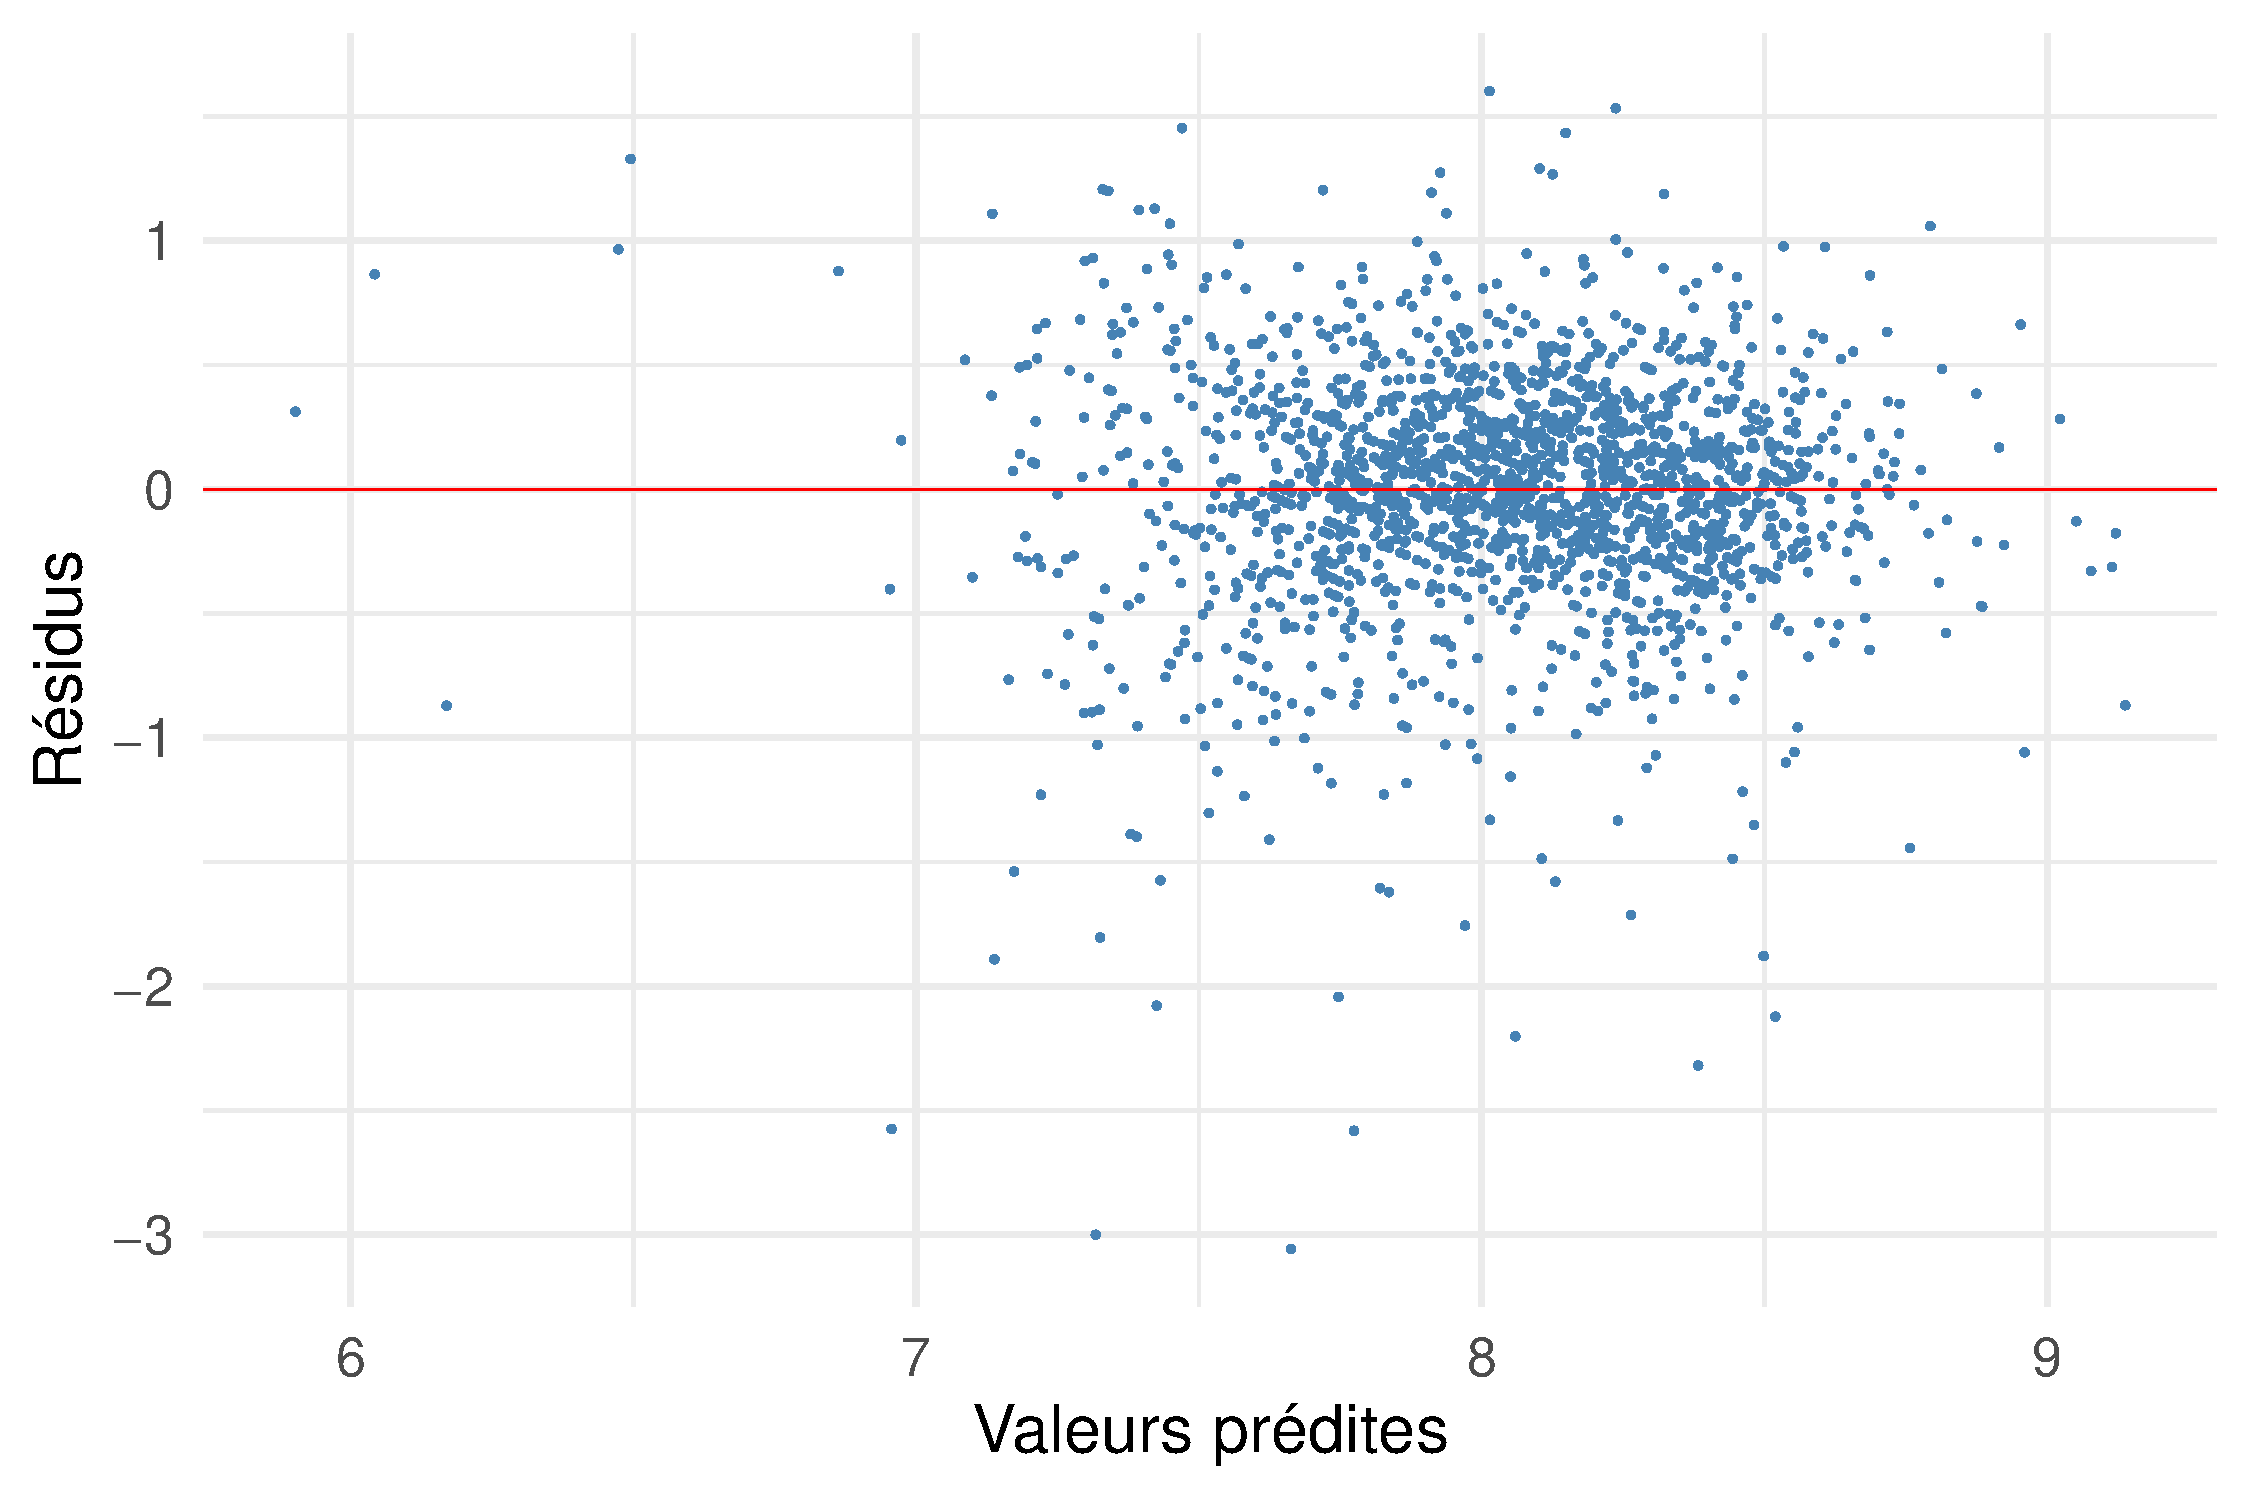
\includegraphics[width=0.49\linewidth]{figure/plot_hetero_fitted.pdf}
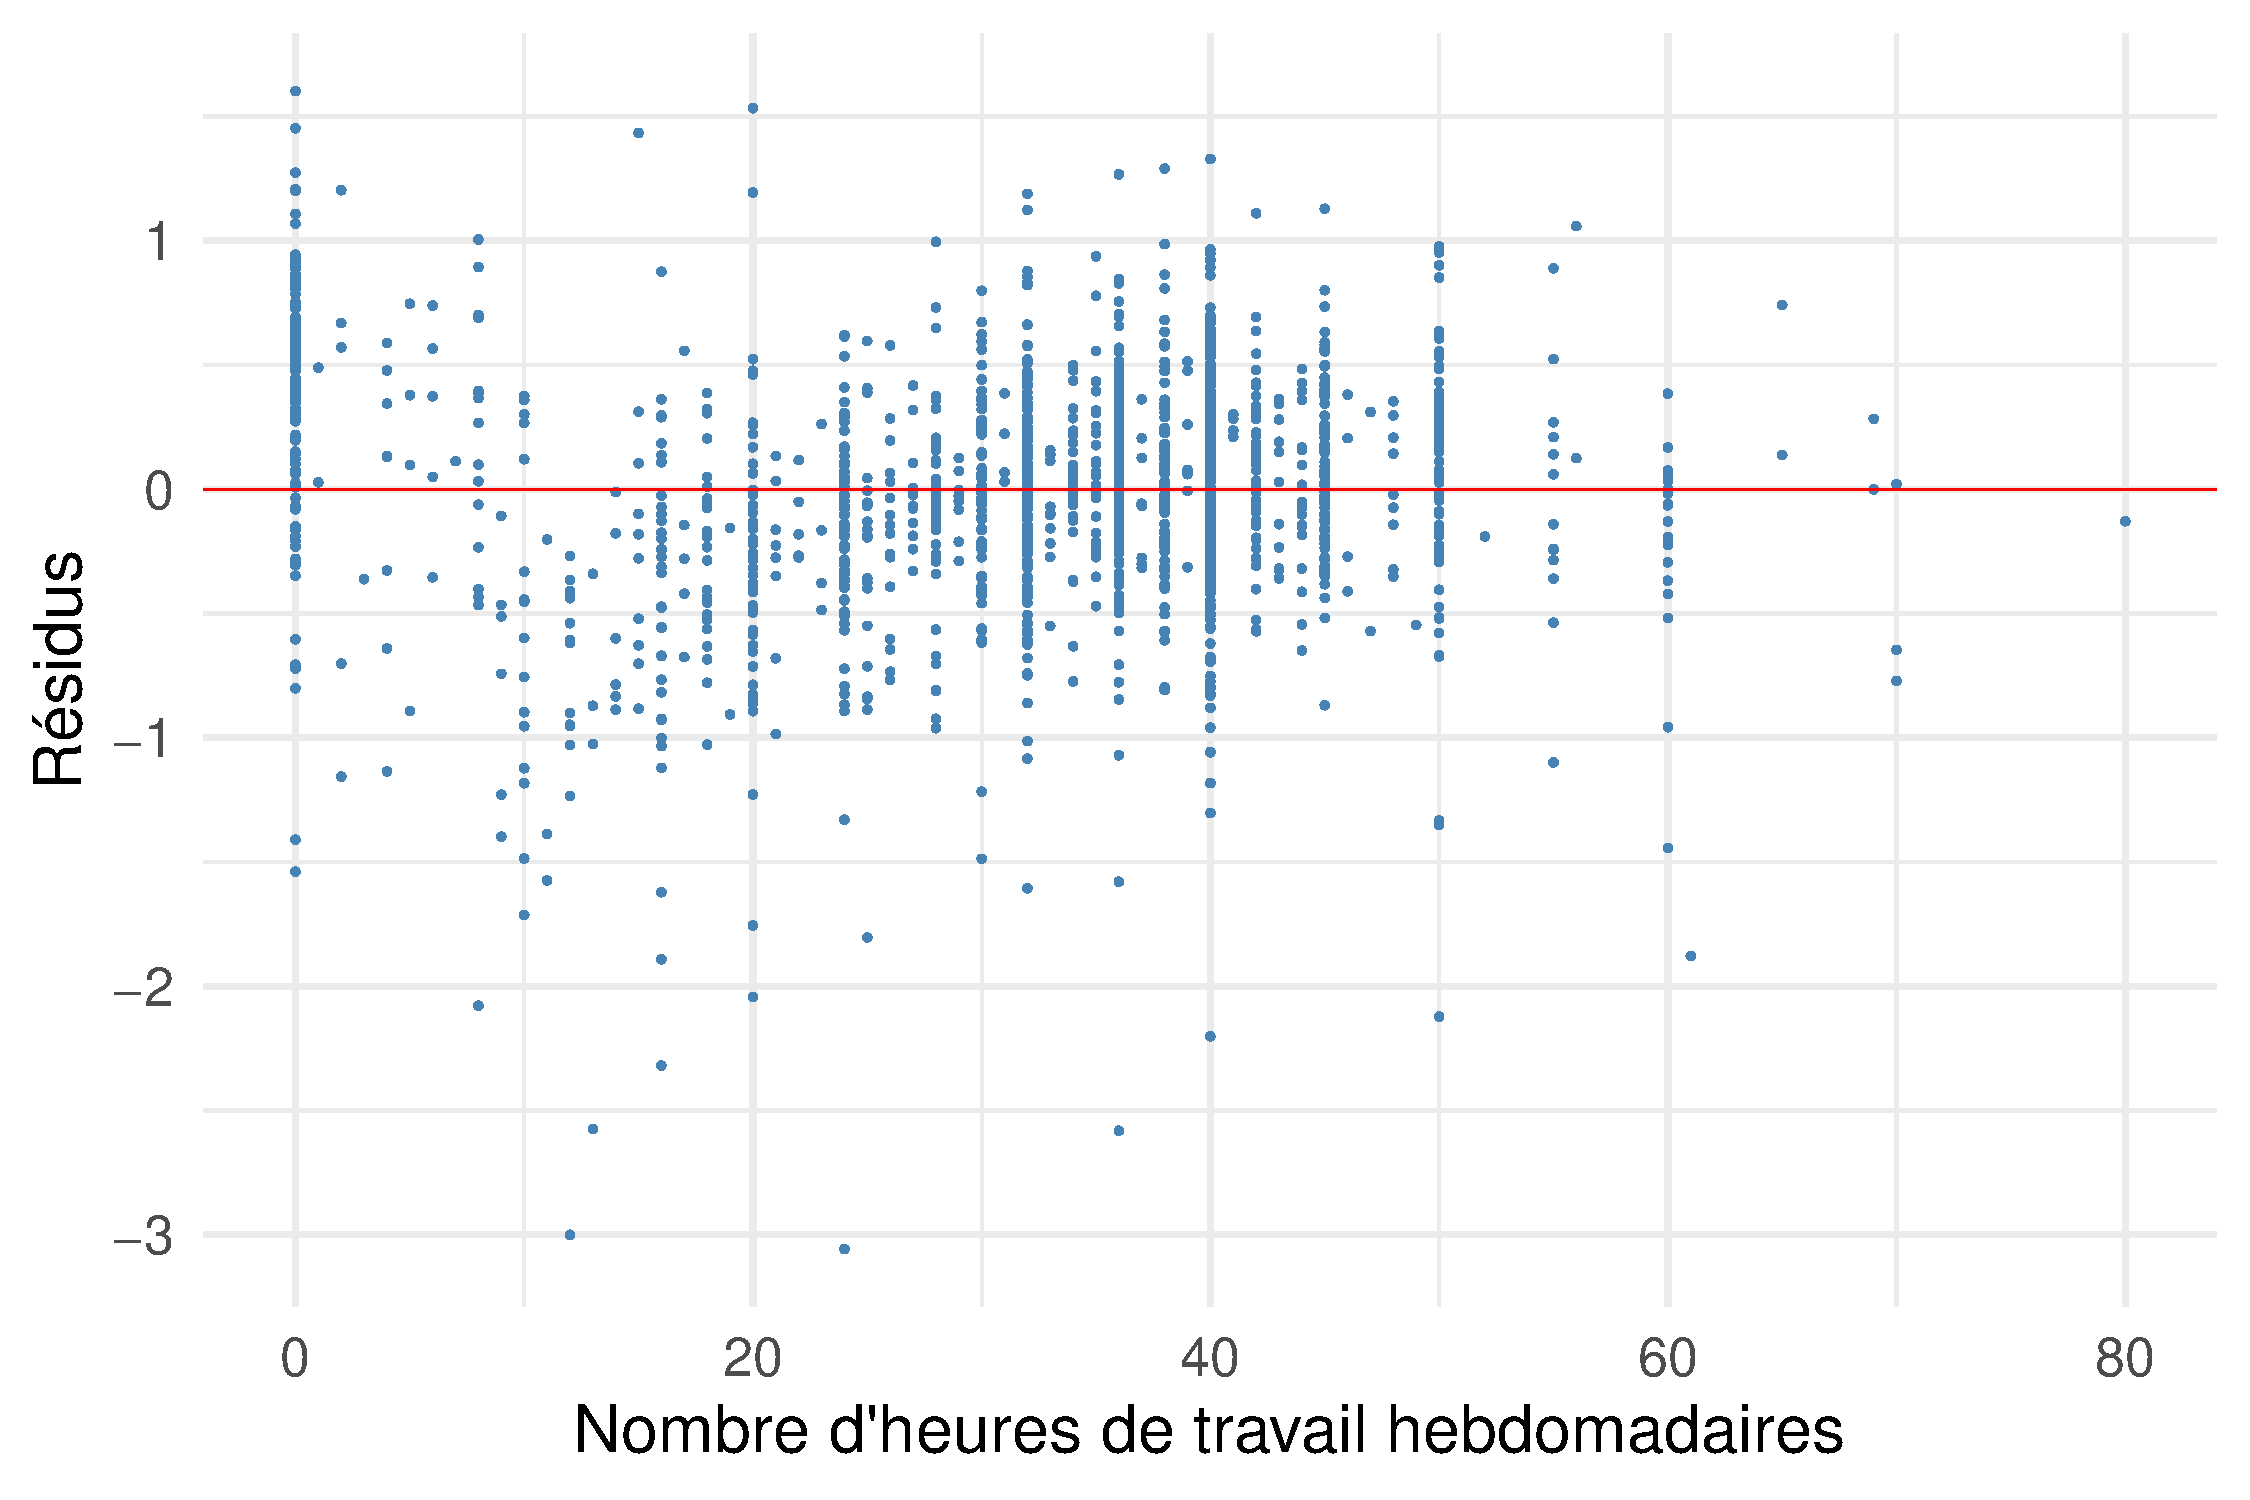
\includegraphics[width=0.49\linewidth]{figure/plot_hetero_heures.pdf}
\caption{Répartition des résidus avant toute correction\label{fig:hetero}}
\end{figure}

Afin de vérifier la présence ou non d’hétéroscédasticité au sein de notre modèle, nous avons réalisé les deux variantes du test de Breusch-Pagan (avec un test de Fisher et avec un test du rapport de vraisemblance) que nous avons également vérifié manuellement pour nous assurer d’obtenir les mêmes valeurs (p-value). Tous concordent et corroborent la présence d’hétéroscédasticité, qui est par ailleurs observable graphiquement : la répartition des résidus en fonction des données prédites n’est pas homogène et l’on observe une forte variabilité de ces résidus en fonction de certaines variables du modèle, notamment la variable heures (graphique~\ref{fig:hetero}) où la dispersion semble être plus forte entre 30 et 40 heures qu’avant ou après. Avec le test de Breusch-Pagan avec le rapport de vraisemblance, dont nous avons vérifié les résultats via la commande \verb+bptest()+, nous obtenons une statistique de 75.6 et une p.value de \ensuremath{2.9\times 10^{-14}}, qui nous permet de rejeter l’hypothèse nulle au seuil significatif de 0,01. 





\begin{figure}[h!]
\center
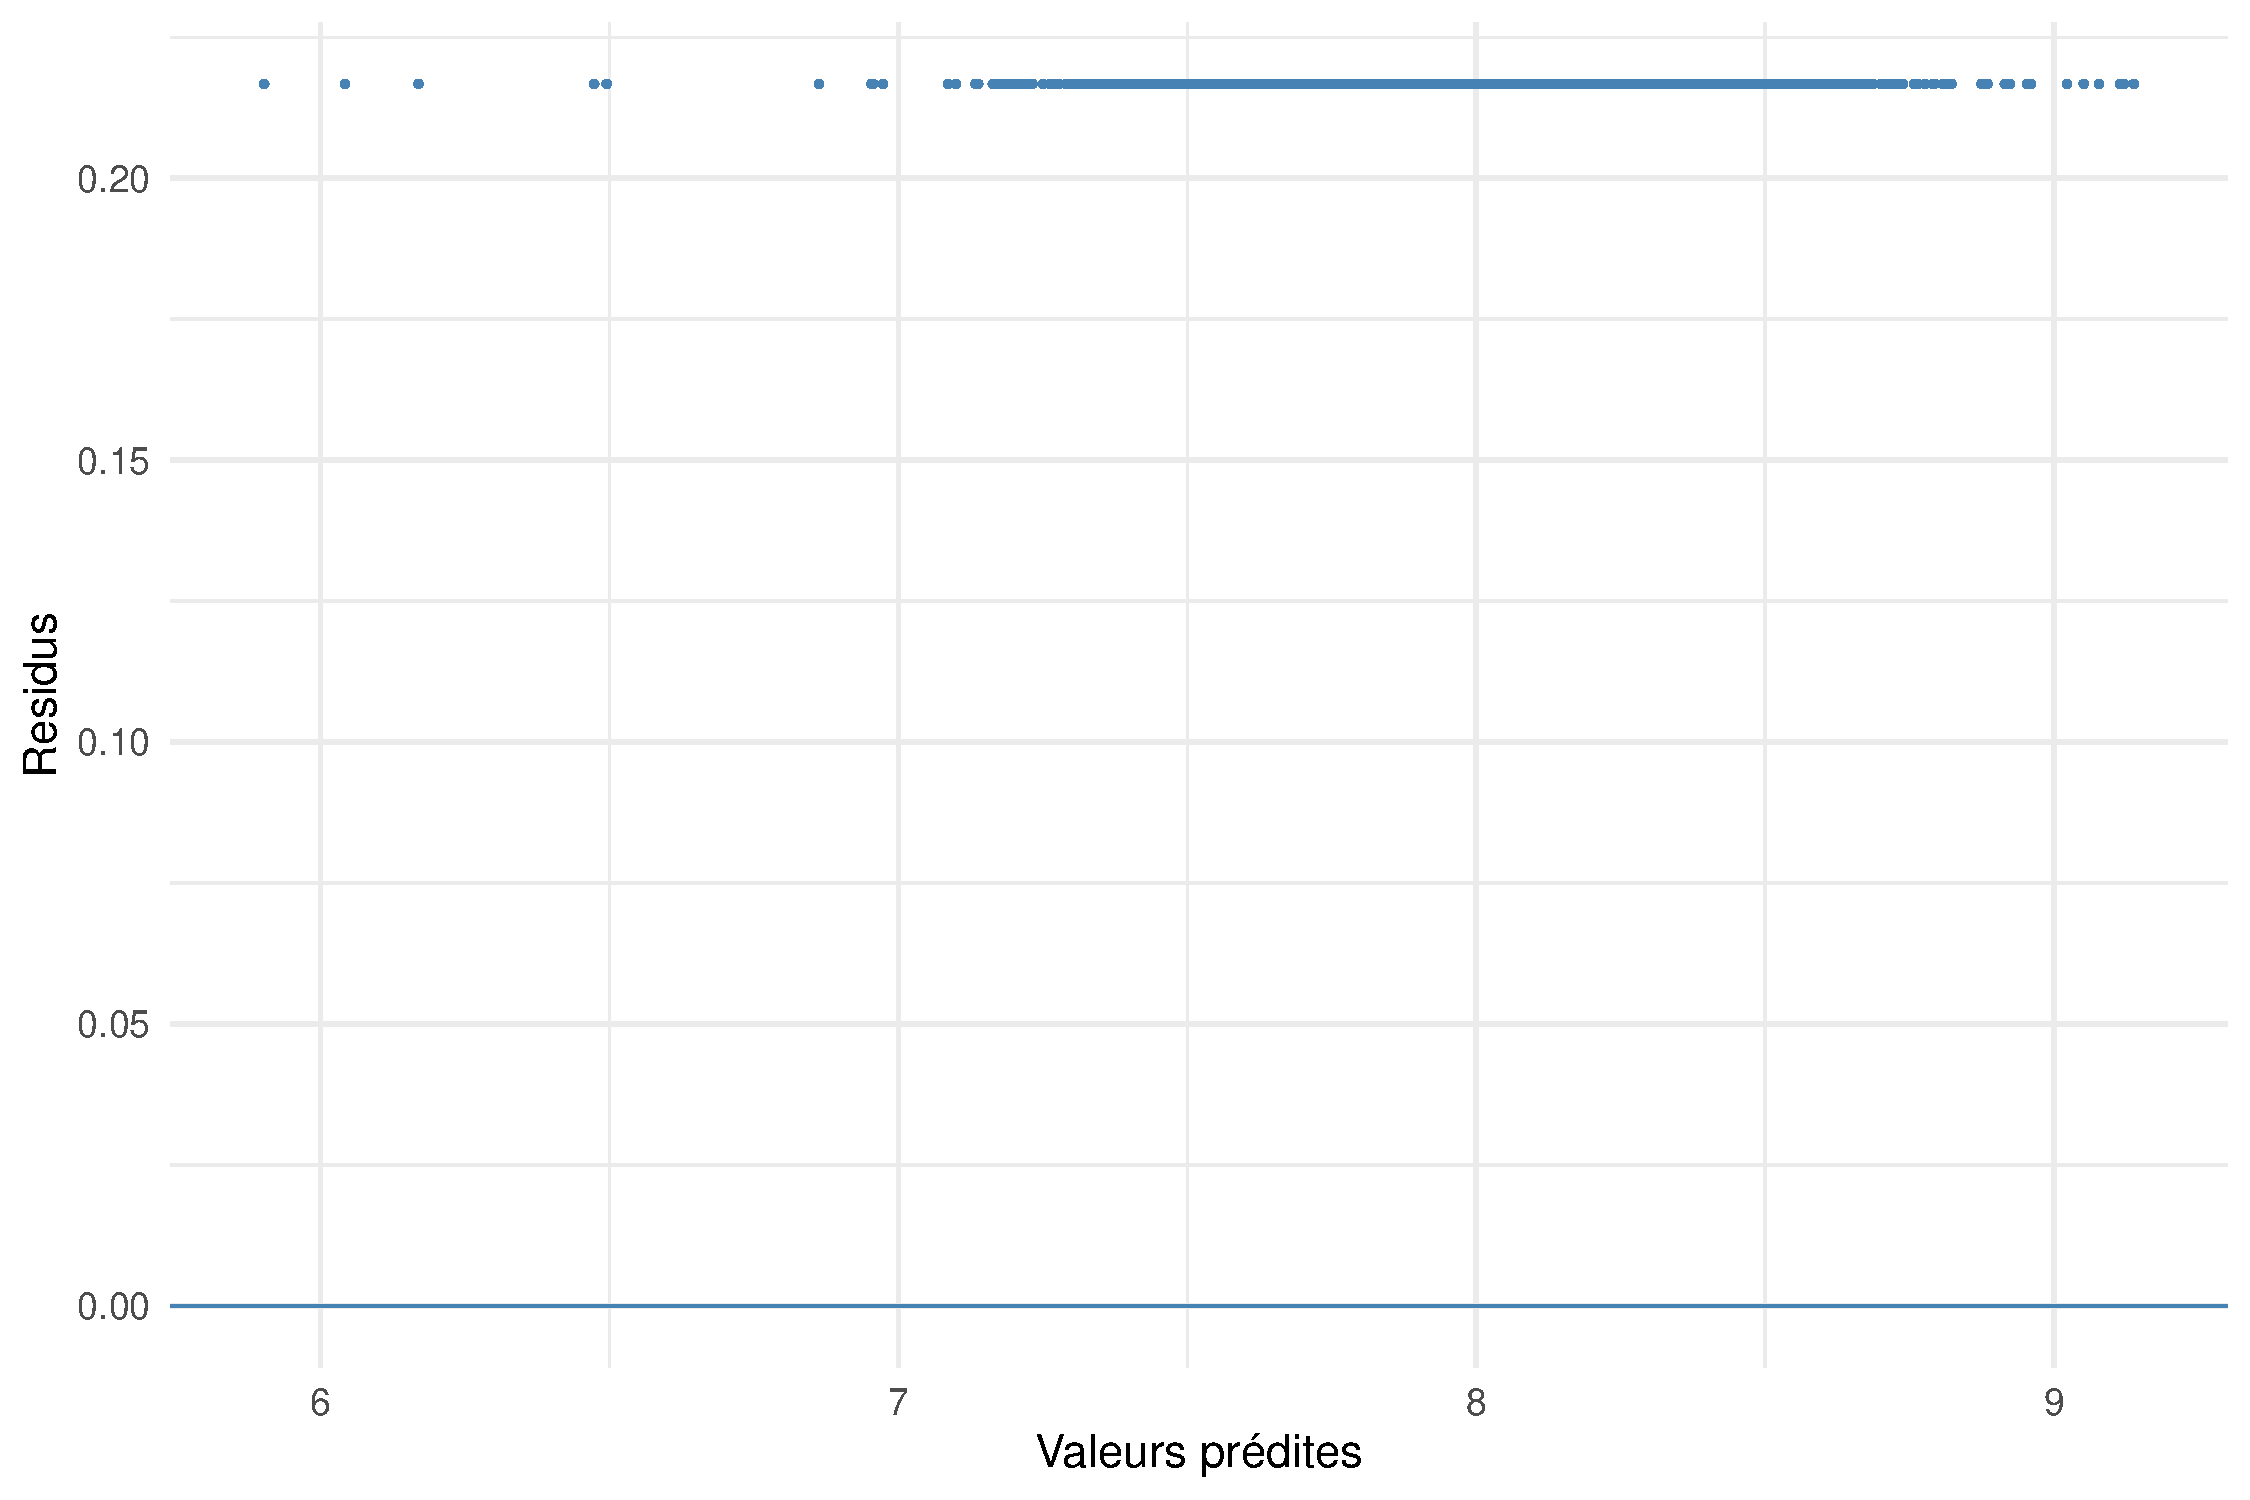
\includegraphics[width=0.7\linewidth]{figure/hetero_correct.pdf}
\caption{Répartition des résidus en fonction des valeurs prédites, après correction de l'hétéroscédasticité\label{fig:hetero_correct}}
\end{figure}

Nous avons corrigé l'hétéroscédasticité en utilisant la méthode de white (variante HC1), via la commande \verb+coeftest+. Après correction, nous obtenons le graphique de répartition des résidus suivant (graphique~\ref{fig:hetero_correct}), confirmant notre correction avec une variance des résidus d’environ 0,22 pour l’ensemble des observations. Nous remarquons dans la régression linéaire classique que les valeurs des paramètres des régresseurs n’ont pas changé, ces dernières n’étant pas influencées par l’hétéroscédasticité. 




\subsection{Détection de l’endogénéité et pistes de correction}

 Une discussion sur la possible présence d’endogénéité dans notre modèle s’impose, dans la mesure où certaines de nos variables, à l'instar d'\texttt{éducation}, ne sont pas exogènes. Si l'on suit l'analyse de Becker, les choix d'éducation --- la poursuite des études, qui représente un investissement financier, ou leur arrêt, qui permet d'entrer sur le marché du travail --- dépendent des ressources des individus. Par conséquent, le nombre d'années d'études dépend au moins pour partie du revenu des parents. Soulignons également l’importance et l’influence du parcours scolaire des parents sur celui de leurs enfants: des parents diplômés pourront inciter leurs enfants à faire des études plus longues, mais surtout les aider (aide aux devoirs notamment). Ce caractère endogène de l'éducation (que l'on pourrait nommer formation initiale) est montré par S. Lollivier et P. Pollet, qui précisent que cette endogénéité conduit, dans leur modèle, \enquote{à majorer d’environ 50 \% l’impact de la formation initiale sur le salaire, ce qui conduit à un gain moyen apparent d’environ 12 \% pour une année d’études supplémentaire contre 8 \% dans l’équation standard} \parencite{lollivier2003}. Malheureusement, nous ne disposions dans notre base de données d'aucune information, ni sur les ressources des parents ni sur leur niveau d'études, qui auraient pu faire des variables instrumentales appropriées. 
 




\begin{figure}[h]
\center
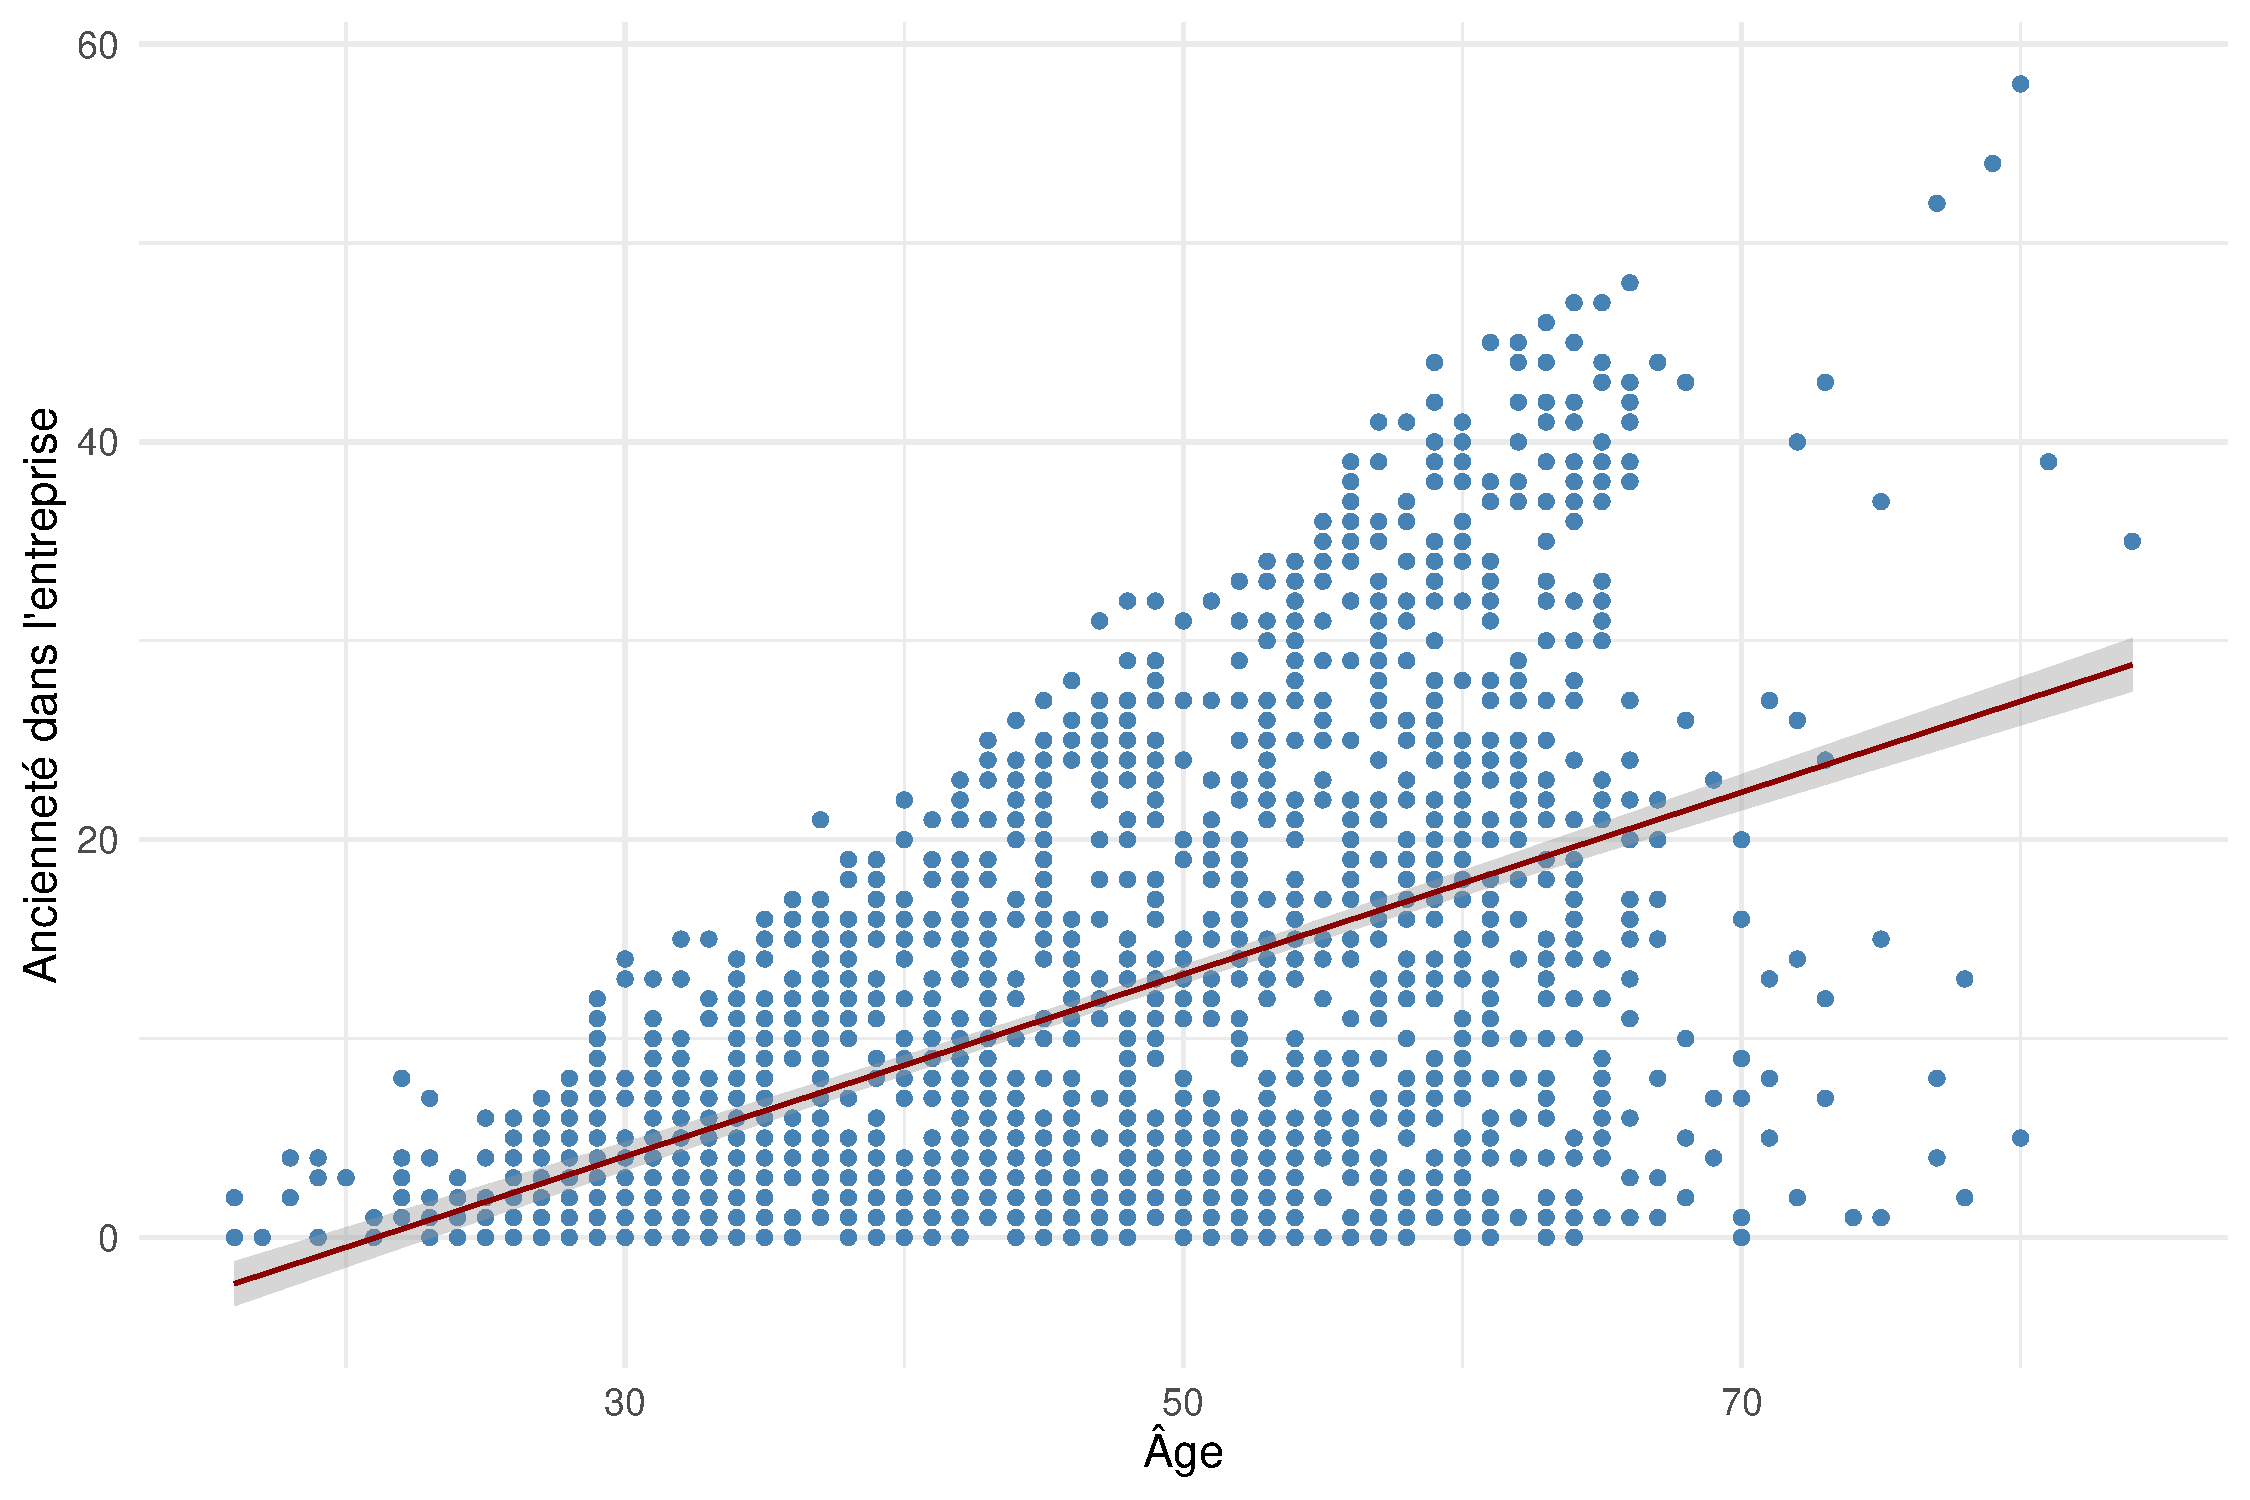
\includegraphics[width=0.7\linewidth]{figure/exp_age.pdf}
\caption{Ancienneté de l'entreprise en fonction de l'âge\label{fig:exp_age}}
\end{figure}

Il nous semble également que l'\texttt{ancienneté} constitue, dans notre modèle, une variable endogène, dans la mesure où elle dépend fortement --- entre autres --- de l'âge. Un individu jeune, de 25 ans par exemple, ne pourra évidemment pas accumuler une dizaine d’années d’ancienneté (voir le graphique~\ref{fig:exp_age}). Cependant, nous ne sommes pas parvenus à trouver une variable instrumentale appropriée dans notre base de données. Nous avons envisagé de contrôler par la variable \texttt{âge}, avant d'y renoncer, parce qu'il nous est impossible de justifier que l'effet de l'âge a un effet sur le revenu uniquement par l'intermédiaire de l'ancienneté dans l'entreprise. Il est au contraire légitime de supposer qu'au-delà de la seule ancienneté --- entendue comme nombre d'années au service de son employeur actuel ---, c'est l'expérience professionnelle ---  par exemple le nombre d'années de travail toutes entreprises confondues --- qui a un impact sur le revenu. C'est d'ailleurs une des limites de notre modèle de ne pas disposer d'une telle variable : en l'absence de variables permettant d'estimer l'expérience des individus, nous n'avons pu que considérer d'une part leur âge et d'autre part leur ancienneté. Enfin, l'effet de l'âge sur le revenu pourrait également être lié à un effet de génération, dans la mesure où certains travailleurs ont pu entrer sur le marché du travail dans un contexte économique plus ou moins favorable, ce qui a pu avoir une influence, à court et à long terme, sur leurs rémunérations. 
        

\section{Résultats principaux}

\subsection{Analyse et discussion des paramètres}

% latex table generated in R 4.2.1 by xtable 1.8-4 package
% Fri May 19 11:45:28 2023
\begin{table}[ht]
\centering
\caption{Paramètres estimés du modèle (hétéroscédasticité corrigée)} 
\label{tb:lm1}
\begin{tabular}{rrrrr}
  \toprule
 & Estimate & Std. Error & t value & Pr($>$$|$t$|$) \\ 
  \midrule
(Intercept) & 5.8617 & 0.1255 & 46.6890 & 0.0000 \\ 
  age & 0.0078 & 0.0012 & 6.7330 & 0.0000 \\ 
  genre & -0.3036 & 0.0223 & -13.6003 & 0.0000 \\ 
  heures & 0.0140 & 0.0011 & 13.0212 & 0.0000 \\ 
  anciennete & 0.0030 & 0.0011 & 2.7550 & 0.0059 \\ 
  nbenfants & -0.0072 & 0.0108 & -0.6637 & 0.5070 \\ 
  education & 0.0922 & 0.0062 & 14.9240 & 0.0000 \\ 
   \bottomrule
\end{tabular}
\end{table}




Nous avons tout d’abord préféré effectuer une analyse en log-niveau, le log limitant les risques d’hétéroscédasticité en \enquote{écrasant} les observations sans les fausser. À première vue, les paramètres de nos 6 régresseurs de base sur la variable expliquée paraissent plutôt cohérents à ce qui est observé dans la littérature, comme le montre le tableau \ref{tb:lm1}, l’âge a une influence positive mais assez négligeable (paramètre de 0,008), le genre a une forte influence négative sur le salaire pour les femmes. Les heures de travail ont évidemment une influence positive forte : 1 heure travaillée en plus par semaine augmente d’environ 1,4\% le log du revenu (voir graphique~\ref{fig:heureslogrevenu}).



\begin{figure}[h]
\center
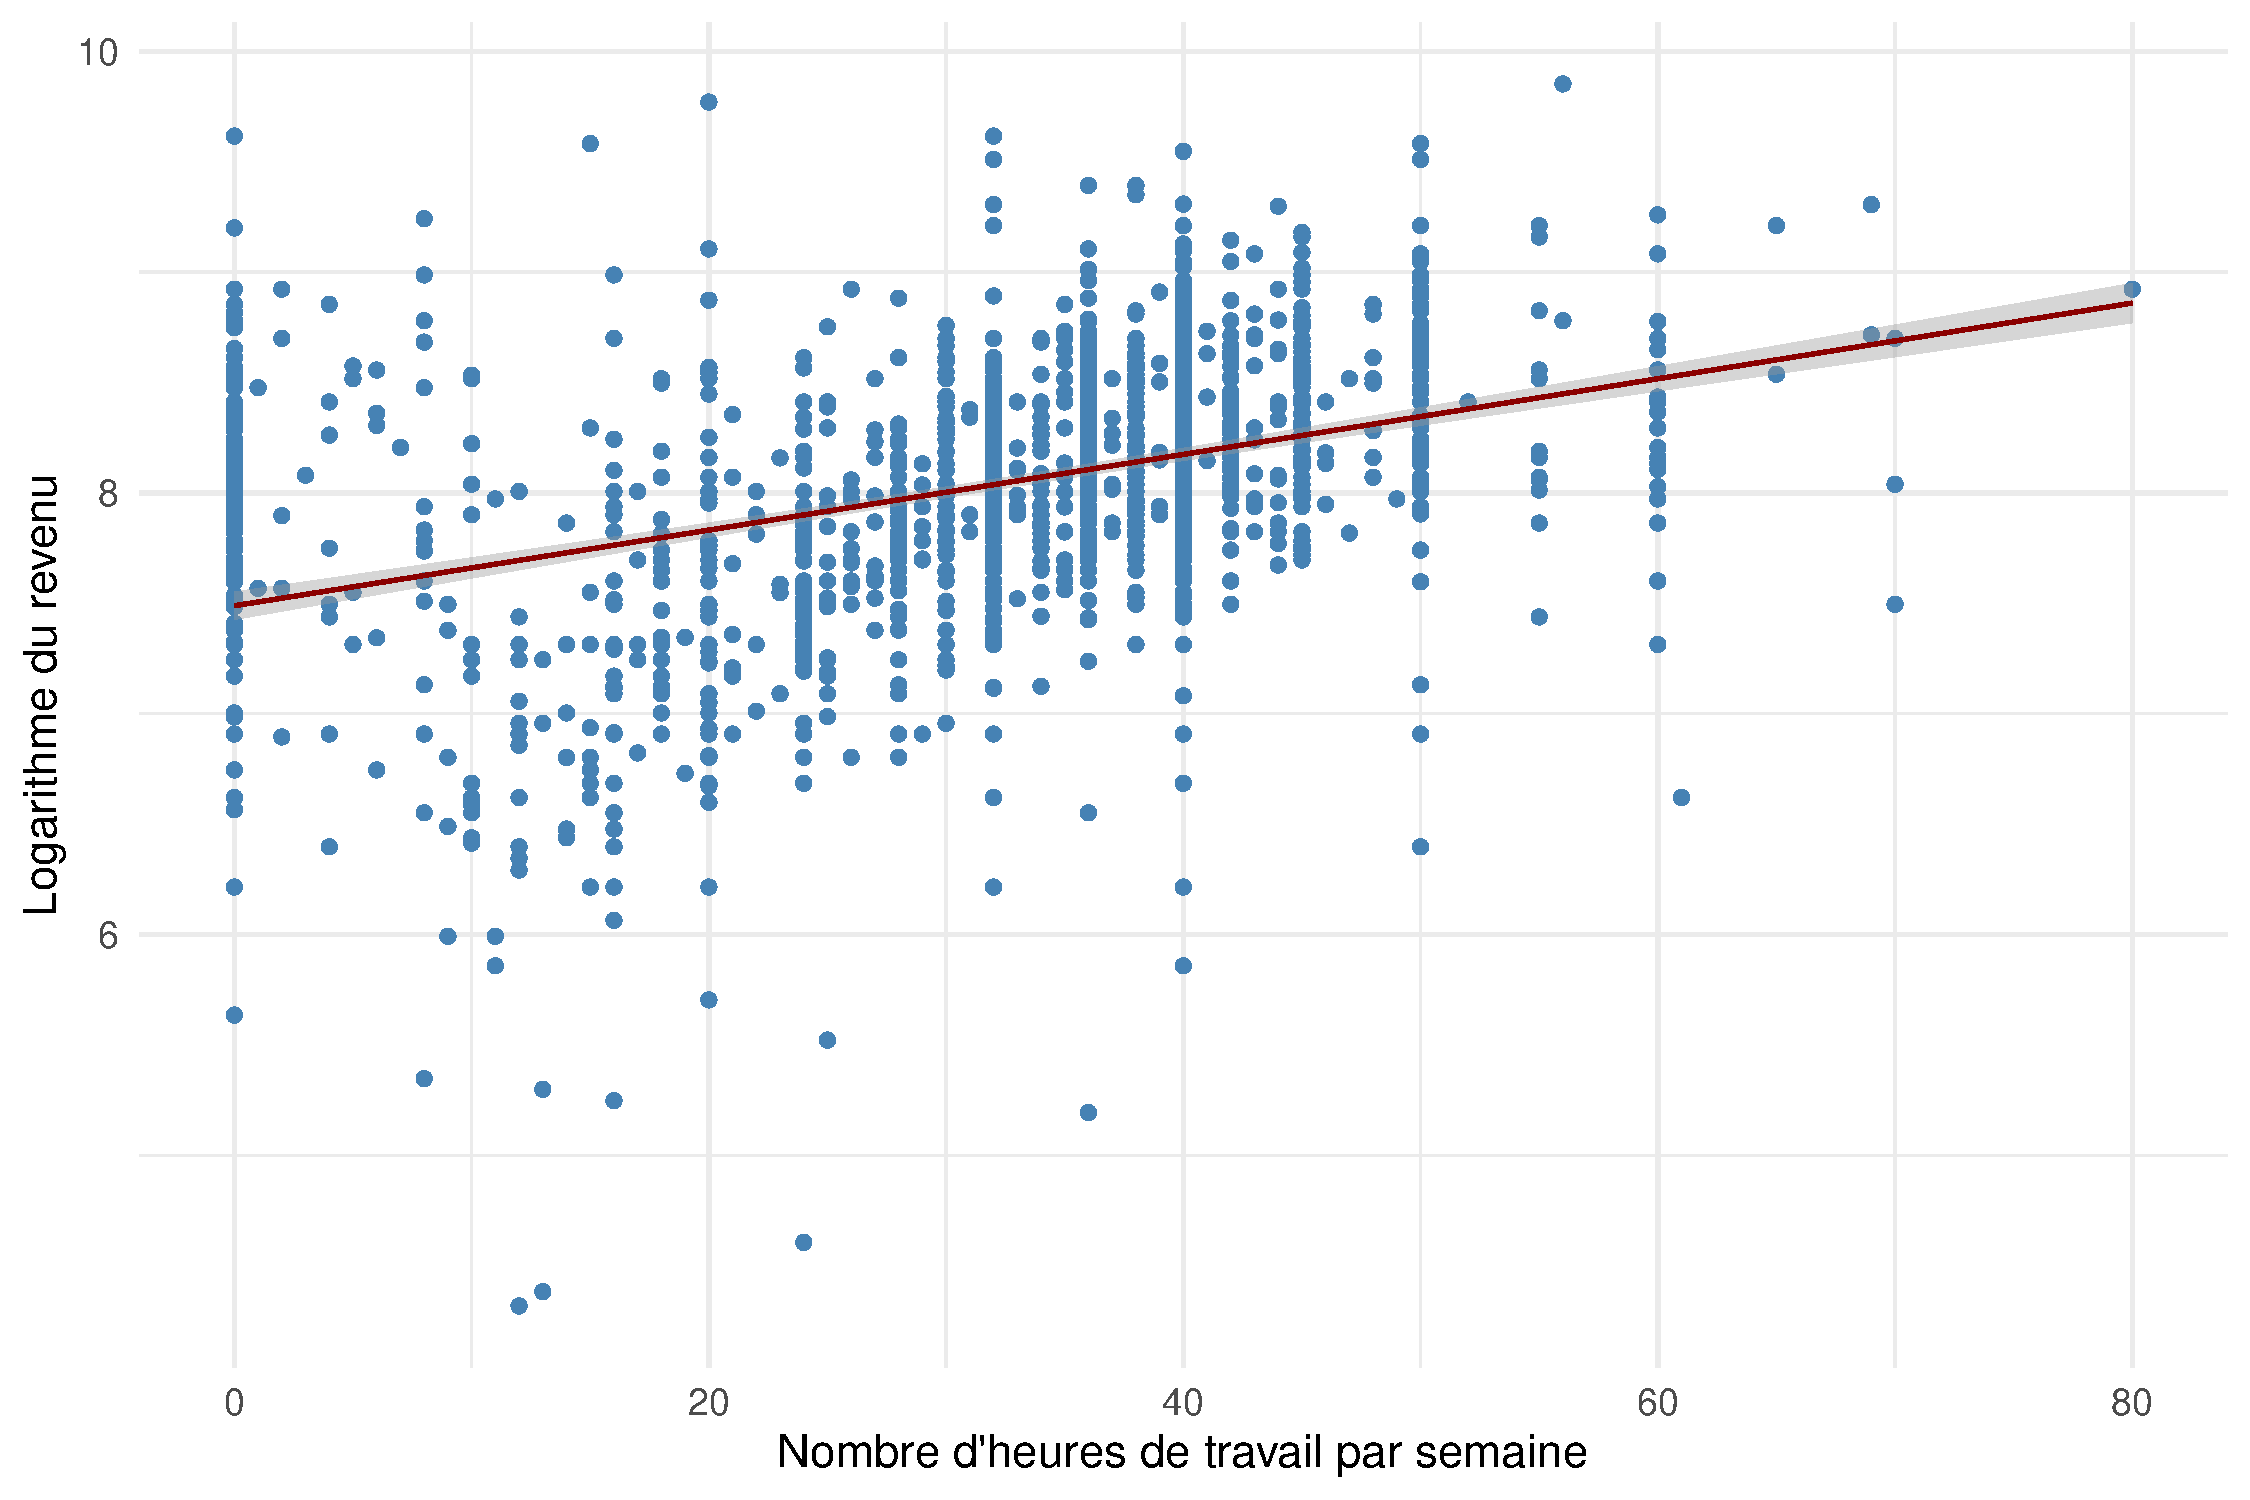
\includegraphics[width=0.7\linewidth]{figure/heures_logrevenu.pdf}
\caption{Log revenu en fonction du nombre d'heures de travail\label{fig:heureslogrevenu}}
\end{figure}

L’ancienneté joue enfin positivement mais faiblement, le nombre d’enfants négativement mais faiblement également, et l’éducation est la variable qui joue le plus fortement avec le nombre d’heures travaillées, avec un paramètre de 0,09. Fait notable, le nombre d’enfants semble assez peu significatif, cette variable étant la seule dans notre régression initiale avec une p-value supérieure à 0,05 (pour atteindre 0,45).
        Les données du LISS semblent donc confirmer à première vue ce que la littérature a déjà pointé du doigt : une différence structurelle de salaire (brut ici) entre hommes et femmes, une influence positive de l’éducation, de l’ancienneté, de l’âge… Ayant souhaité nous concentrer plus particulièrement sur l’effet de l’éducation, nous avons cependant souhaité vérifier l’existence d'effets de seuils de l’éducation sur le salaire au moment de l’obtention d’un diplôme. Nous allons désormais évoquer les résultats d’un test de Chow effectué sur l’éducation. 

\subsection{Test de chow sur la variable \texttt{éducation}}



L’intérêt de cette partie est d’identifier un éventuel niveau d’études qui fait rupture dans le modèle en menant un test de Chow sur la variable \texttt{éducation}. Nous avons décidé de tester l’existence d’un changement structurel dans notre modèle au-delà de 16 ans d’études. Il s’agit de savoir si notre modèle est stable au sein de deux sous-populations, qui se distinguent par la durée de leur scolarité et de leurs études. Notons qu’ici peu importe que l’égalité soit stricte ou pas, étant donné qu’\texttt{éducation} n’est pas continue. Formellement, en écrivant notre modèle comme suit :

\[Y = \beta_1X_1 + \beta_2X_2 + \dots + \beta_6X_6\] 

\noindent où $\beta_i$ est le coefficient associé au régresseur $X_i$, nous testons l'hypothèse nulle $H_0$ contre l'hypothèse alternative $H_1$ :

\[\begin{cases} H_0 &: \forall i=1, \dots, 6, \quad\beta_{i_{\texttt{\tiny éducation}<16}}=\beta_{i_{\texttt{\tiny éducation}>16} }= \beta_i \\ H_1 &: \exists i=1,\dots,6\ / \quad \beta_i\neq \beta_{i_{\texttt{\tiny éducation}<16}} \text{ ou } \beta_i\neq\beta_{i_{\texttt{\tiny éducation}>16} } \end{cases}\]



Avec $\beta_{i_{\texttt{\tiny éducation}<16} }$ les coefficients du régresseur $X_i$ pour la sous-population la moins diplômée. Les effectifs de nos deux sous-populations sont de tailles suffisantes (1076 personnes d'un côté (les plus diplômés) et 831 personnes de l'autre). Le test (réalisé manuellement, puis confirmé avec la commande \texttt{sctest()}) nous donne une statistique de 12.2 et une p-value de \ensuremath{2.6\times 10^{-15}}, nous pouvons donc conclure à l'existence d'un changement structurel dans la relation entre nos régresseurs et le log revenu entre l'échantillon des moins diplômés et celui des plus diplômés. Pour analyser plus finement ce changement, examinons les tableaux des paramètres estimés pour nos deux sous-groupes. 

\begin{table*}[htbp]
\captionof{table}{\centering Paramètres estimés du modèle pour les sous-groupes des moins diplômés (à gauche) et des plus diplômés (à droite)}\label{tab:chow}
   \begin{minipage}[t]{0.4\linewidth}
   {\tiny
      \centering
\begin{tabular}{rrrrr}
  \toprule
 & Estimate & Std. Error & t value & Pr($>$$|$t$|$) \\ 
  \midrule
(Intercept) & 6.5637 & 0.1422 & 46.1515 & 0.0000 \\ 
  age & 0.0047 & 0.0015 & 3.1557 & 0.0017 \\ 
  genre & -0.3778 & 0.0336 & -11.2534 & 0.0000 \\ 
  heures & 0.0137 & 0.0012 & 11.3171 & 0.0000 \\ 
  experience & 0.0055 & 0.0015 & 3.6817 & 0.0002 \\ 
  nbenfants & -0.0334 & 0.0140 & -2.3833 & 0.0174 \\ 
  education & 0.0512 & 0.0082 & 6.2682 & 0.0000 \\ 
   \bottomrule
\end{tabular}}
   \end{minipage}
   \hspace{2cm}
   \begin{minipage}[t]{0.4\linewidth}
   {\tiny
      \centering
\begin{tabular}{rrrr}
  \toprule
Estimate & Std. Error & t value & Pr($>$$|$t$|$) \\ 
  \midrule
6.2337 & 0.2089 & 29.8446 & 0.0000 \\ 
0.0106 & 0.0013 & 7.9129 & 0.0000 \\ 
-0.2523 & 0.0288 & -8.7473 & 0.0000 \\ 
0.0138 & 0.0011 & 12.5308 & 0.0000 \\ 
0.0003 & 0.0016 & 0.2059 & 0.8369 \\ 
0.0169 & 0.0126 & 1.3477 & 0.1781 \\ 
0.0660 & 0.0109 & 6.0709 & 0.0000 \\ 
   \bottomrule
\end{tabular}}
   \end{minipage}
   \hfill
\end{table*}

En quelques mots, on remarque à la lecture du tableau~\ref{tab:chow} que l'effet du genre sur le salaire est bien plus faible chez les plus diplômés, ce qui peut s'expliquer par des règles plus strictes pour encadrer les salaires (fonction publique) et par une plus grande part de femmes au sein des métiers occupés par les plus diplômés, chaque année d'éducation est également légèrement plus valorisée pour les plus diplômés, de même que l'âge. On note également une rupture au niveau des effets du nombre d'enfants : si la variable joue négativement chez les moins diplômés (chaque enfant en plus tend à faire baisser le salaire de 3,3\%), à l'inverse elle joue positivement chez les plus diplômés (chaque enfant tend, selon le modèle, à une hausse du salaire de 1,7\%).

\section{Mise en perspective des résultats et pistes de prolongement}

\subsection{Un modèle aux ambitions limitées}

Une première limite tient au choix d’utiliser des données en coupe instantanée : notre modèle se borne donc à rendre compte d'une situation à un moment donné sans préjuger de ses évolutions ni passées ni futures. Or comme le soulignent S. Lollivier et P. Pollet, les données issues de coupes instantanées peuvent être affectées par des phénomènes conjoncturels, sans qu'il soit possible d'en déterminer les effets, ce qui restreint la portée de l'analyse \parencite{lollivier2003}. Comment interpréter par exemple une crise économique ou une vague de licenciements massifs ? Ou une nouvelle loi sur le temps de travail ? Pour nos données (qui datent de 2022), ce pourrait être la guerre en Ukraine qui influerait sur certains secteurs, en poussant à la hausse ou à la baisse les salaires. Mais au-delà, les données en coupe instantanée ne permettent pas de mesurer l'évolution de l'influence de certaines variables explicatives, ce qui permet pourtant de dégager des dynamiques de long terme.   L'étude réalisée par D. Witkowska sur les déterminants des salaires en Pologne de 2001 à 2009 est à cet égard exemplaire. Elle y montre montre qu'entre 2001 et 2009, l'écart entre la part de la rémunération imputable aux études chez les personnes ayant été à l'université d'une part et d'autre part chez celles et ceux s’étant arrêté avant \textit{(general secondary} ou \textit{post secondary)} tend à se réduire : le paramètre pour les individus ayant été jusqu’à l’université était 4 fois plus élevé en 2001 que ceux s’étant arrêté au lycée ; en 2009 le rapport n’était plus que de 2 \parencite[p. 206]{witkowska2014} (précisons que ceci ne signifie pas que les individus ayant été à l’université gagnent deux fois plus que les autres, d’une part le salaire est en log et d’autre part cela représente seulement les différences de salaire imputables à l’éducation).

Une autre limite tient au faible nombre de variables explicatives, qui sont pour certaines incomplètes. Il serait préférable de considérer l'expérience plutôt que l'ancienneté, et le modèle y gagnerait certainement, mais nous ne disposions pas d'une telle variable. Un autre facteur intéressant aurait pu être l'existence de périodes de chômage mais aussi de découpler salaire et autres revenus (autrement dit, revenus du travail et revenus du capital).  D'autres variables auraient pu être envisagées, telles que le type de contrat ou encore la taille de l'entreprises, qu'utilise D. Witkowska dans son article, mais à nouveau se posait le problème des contraintes induites par notre base de données. Néanmoins, nous avons effectué en amont un travail de présélection des variables, qui nous a conduit à éliminer celles qui n'étaient pas suffisament significatives. Il aurait été intéressant de présenter ici les résultats de la régression, mais il était nécessaire d'écarter ces variables, sauf à voir la taille de l'échantillon diminuer trop fortement. Sans plus de détails, nous pouvons mentionner quelques unes de ces variables peu significatives : le travail en soirée ou de nuit ; le lieu de résidence (rural ou urbain) ; le fait d'avoir posé récemment des congés ; l'état de santé ; la présence d'enfants de moins de huit ans ; la situation matrimoniale.  



\subsection{Élargir le périmètre d'investigation}

Mais, au-delà de de l'intégration d'évolutions temporelles ou de nouvelles variables, l'une des principales pistes de prolongement de ce travail réside probablement dans un élargissement de la notion de revenu. Nous avons en effet considéré le revenu à un moment donné (la variable utilisée ne précise pas qu'il s'agit d'une moyenne, il est donc raisonnable de supposer qu'il s'agit du dernier salaire perçu au moment de l'enquête). Or ce paramètre ne permet pas de rendre compte des éventuelles variations à court, voire très court terme de revenu, en particulier pour celles et ceux dont les contrats sont atypiques. Pour compléter l'analyse, une prise en compte de la stabilité --- ou, \textit{a contrario}, de la volatilité --- du revenu serait bienvenue dans la mesure où le revenu n'est pas une fin en soi. Il est un objet d'analyse priviligié en ce qu'il témoigne non seulement d'un statut social, mais également de possibilités de consommations dont dépendent fortement l'utilité des individus. Dans ce cadre, il est évident que la régularité des revenus est déterminante aussi bien s'agissant du statut social que du niveau de consommation. Ajoutons qu'il s'agit d'un critère institutionnalisé dans la mesure où les banques ne consentent généralement des prêts qu'aux personnes ayant des revenus stables. 

Ceci rejoint les propos de S. Lollivier et P. Pollet qui recommandent de prendre en compte, en plus du revenu, les opportunités d’emploi et le fait de ne pas se retrouver au chômage. Des formations différentes donnent, selon eux, des accès et opportunités différentes d’accès à l’emploi qui ne sont pas pleinement retranscrites par le biais du salaire. Pour un même salaire, des individus dans des branches différentes d’emploi peuvent avoir une certitude tout à fait différente quant à la stabilité de leur poste ou des possibilités d’embauche futures. Il pourrait donc s'agir d'intégrer la probabilité d'être au chômage dans l'analyse (par exemple en tenant compte du nombre de périodes de chômage passées et de leur durée), voire de pondérer le salaire mensuelle par un indice dépendant de ses variations (ex : variance du salaire mensuel par rapport à la moyenne anuelle). 

\section*{Conclusion}
         
         Notre contribution, qui vient en grande partie corroborer des résultats précédemment établis ouvre néanmoins la voie à des axes de recherche originaux. S'il ne s'agit certes que d'un instantané, d'une présentation de l'influence de différents paramètres sur le salaire brut à un moment donné, certains résultats de notre modèle n'en sont pas moins intéressants. Ainsi du paramètre estimé du genre, qui joue à hauteur de -30\% du salaire pour les femmes : si l'écart de salaire --- net --- entre hommes et femmes semble davantage se situer aux environs de 13.5\%\footnote{\url{https://www.statista.com/statistics/1371618/benelux-gender-pay-gap/}}, notre résultat, au-delà des spécificités éventuelles inhérentes à la base de données, montre l'ampleur de l'écart lorsque l'on considère le brut --- en particulier dans des États dont la fiscalité progressive a tendance a estomper les différences de rémunération. Par ailleurs, il est intéressant de noter que ce \textit{gender pay gap} varie en fonction du niveau d'études, les différences étant plus marquées chez les moins diplômés (voir tableau \ref{tab:chow}). Sur le plan de la méthode, il pourrait être intéressant dans le cadre d'une étude plus approfondie, de réaliser des régressions linéaires en différenciant systématique les coefficients en fonction des sous-groupes (différenciés à partie du genre, du niveau de diplôme, etc) afin obtenir des résultats plus fins et plus aisément comparables vis-à-vis de la littérature existante. 

\vspace{0,3cm}

Toutes nos analyses ont été réalisées à l'aide du logiciel statistique R (version 4.2.1, R Core Team 2022). Les différents paquets utilisés sont listés en page~\pageref{sec:ref}. Ce document a été écrit avec \LaTeX. 

\nocite{*}
\printbibliography[notkeyword={Rsoftware}, title={Bibliographie}]

\printbibliography[keyword={Rsoftware}, title={Logiciels et paquets}]
\label{sec:ref}

\appendix
\appendixpage
\addappheadtotoc

\section{Précisions sur les variables utilisées et leur codage}

\subsection{La variable \texttt{age}}

Il s’agit de la variable \texttt{leeftijd}, issue du questionnaire \textit{Background variables}, reprise telle quelle. Les valeurs vont de 16 à 84 ans. 

\subsection{La variable \texttt{education}}

Il s'agit du regroupement de deux variables : nous avons d'abord récupéré les données de la variable \texttt{oplmet} du questionnaire \textit{Background variables} et avons converti les différentes modalités en nombre d'années d'éducation (scolarité et études), comme suit : 

\vspace{0,5cm}
\begin{minipage}{0,8\linewidth}
{\footnotesize\texttt{oplmet} : Highest level of education with diploma
\vspace{0,2cm}

\begin{tabular}{m{0,5\linewidth}m{0,5\linewidth}}
\hline
Valeur d'origine & Valeur de remplacement \\
\hline
1. primary school [8 ans] & 8 (de 4 à 12 ans) \\
2. vmbo (intermediate secondary education, US: junior high school) [4 ans] & 12 (après l'école primaire) \\
3. havo/vwo (higher secondary education/preparatory university education, US: senior high school) [5-6 ans] & 13.5 (après l'école primaire) \\
4. mbo (intermediate vocational education, US: junior college) [1-4 ans] & 15.25 (après VMBO, HAVO ou VWO, soit en moyenne 2.5 + 12.75)\\
5. hbo (higher vocational education, US: college)[4 ans] & 16.75 (après VMBO, HAVO ou VWO, 4 + 12.75)\\
6. wo (university) [3 ans]& 17 (après 1ere année HBO ou après VWO, 14 + 3)\\
7. other & suppression des observations \\
8. Not (yet) completed any education & 0 \\
9. Not yet started any education & 0 \\
\hline
\end{tabular}}
\end{minipage}
\vspace{0,3cm}

La variable \texttt{oplmet} ne proposant pas de modalité \textit{master} ou \textit{Ph.D.}, nous nous sommes ensuite appuyés sur la variable \texttt{cw22o005} du questionnaire \textit{Work and schooling}. Cette variable, très complète, comprend 28 modalités, ce qui la rendait trop difficile à coder étant donné que nous ne maîtrisons pas les subtilités du système universitaire néerlandais, mais nous nous sommes contentés de récupérer les trois modalités qui nous intéressent, afin de compléter le codage de la variable \texttt{education}, comme suit : 

\vspace{0,5cm}
\begin{minipage}{0,8\linewidth}
{\footnotesize\texttt{cw22o005} : What is the highest level of education that you have completed with diploma or certificate?
\vspace{0,2cm}

\begin{tabular}{m{0,5\linewidth}m{0,5\linewidth}}
\hline
Valeur d'origine & Valeur de remplacement \\
\hline
25. academic education, bachelor [3 ans] & 17 (soit la valeur que nous avions déjà) \\
26. academic education, master [1-3 ans] & 19 (17 +2) \\
27. doctor's degree (Ph.D, including doctoral research program to obtain Ph.D) [3-4 ans] & 22.5 (19+3.5) \\
\hline
\end{tabular}}
\end{minipage}
\vspace{0,3cm}

À l'issue du codage, on obtient la répartition suivante : 

\begin{figure}[h]
\center
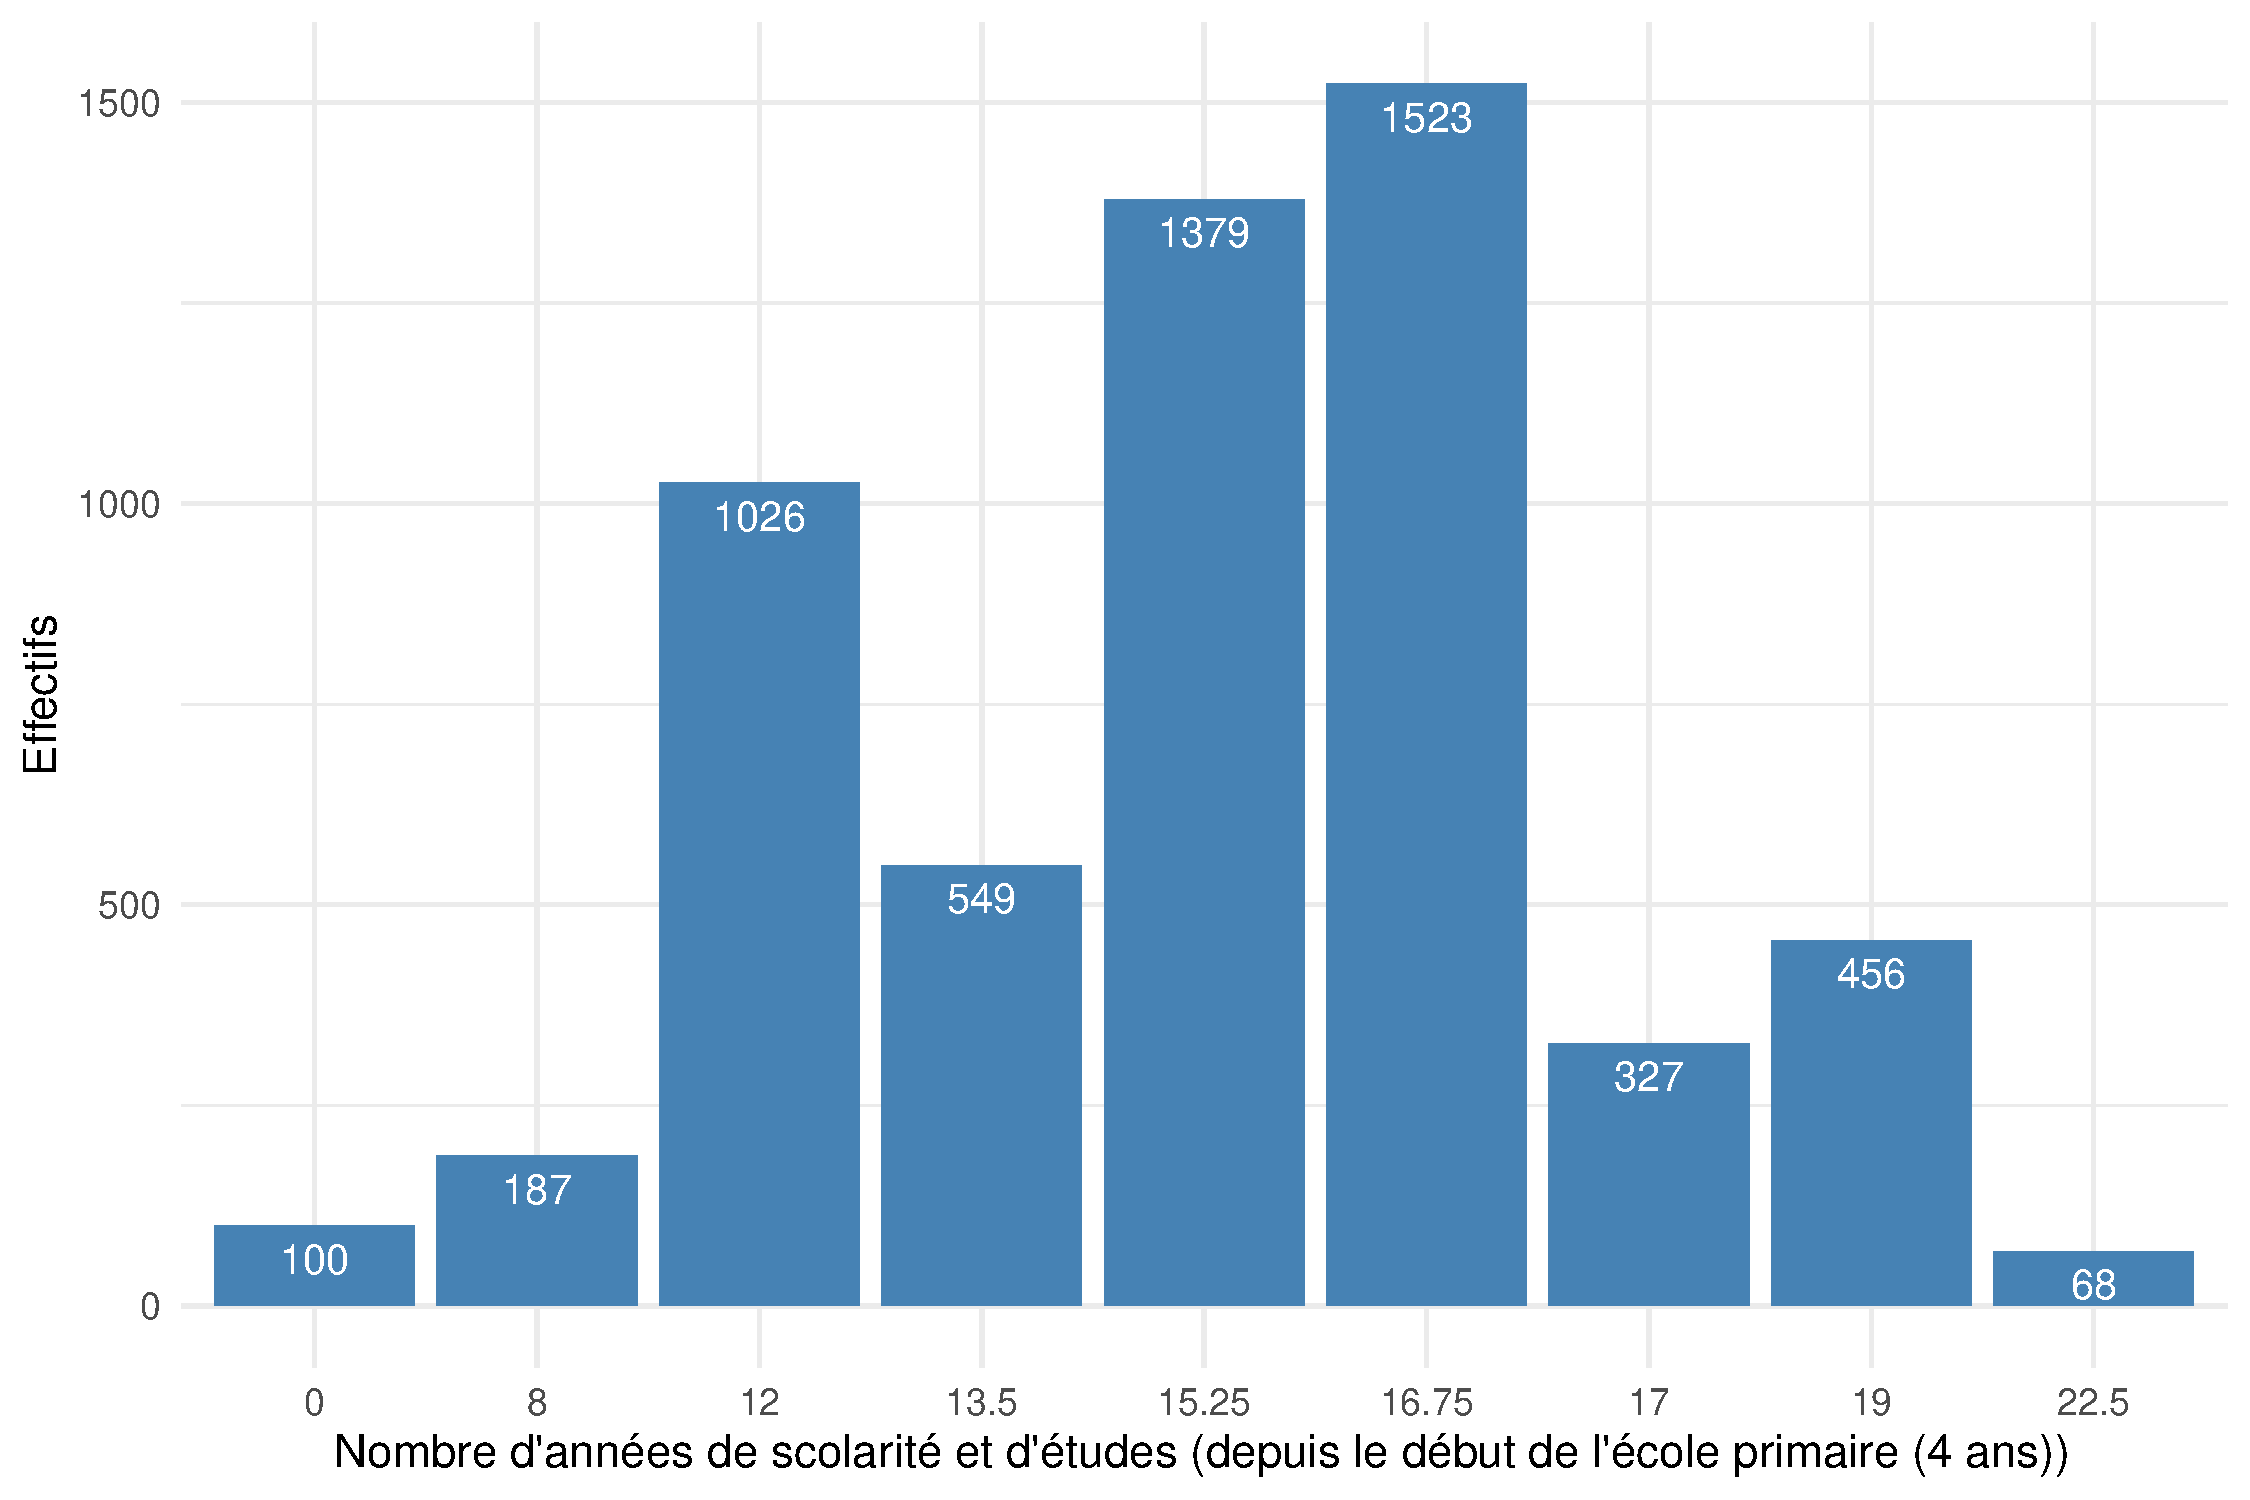
\includegraphics[width=0.7\linewidth]{figure/educ.pdf}
\caption{Niveau d'éducation (avec diplôme) des individus de l'échantillon}
\end{figure}

\subsection{La variable genre}

Cette variable est issue de la variable \texttt{geslacht} du questionnaire \textit{Background variables}, dont nous avons enlevé toutes les réponses autres (ni masculin, ni féminin), qui sont par ailleurs très minoritaires (4 observations, soit moins de 0,1\% des observations)

\subsection{La variable revenu}

Issue de la variable \texttt{brutoink} du questionnaire \textit{Background variables}, elle correspond au revenu brut mensuel individuel (\textit{personal gross monthly income}), dans notre modèle, nous utilisons principalement le logarithme de cette variable (\verb+log_revenu+). Nous avons décidé de supprimer les observations pour lesquelles le revenu déclaré est nul, suivant l'avertissement présent dans le \textit{codebook} du LISS : 

\begin{quote}
\textcolor{gray}{Since some people prefer not to make their income information available to Centerdata, a 0 (zero) can mean two different things: (1) that there is no income at all, or (2) that a panel member does not know what the income is or does not want to make that information available to us.}
\end{quote}

\subsection{La variable heures}

Il s'agit de la variable \texttt{cw22o127} du questionnaire \textit{Work and schooling}, qui correspond à la question : \enquote{How many hours per week do you work on average? / How many hours per week did you work on average?}, que nous avons reprise telle quelle. Les valeurs s'échelonnent de 0 à 80 heures hebdomadaires, avec une médiane égale à 36 heures.

\subsection{La variable \texttt{ancienneté}}

Issue du questionnaire \textit{Work and schooling} (variable \texttt{cw22o134}), il s'agit de la réponse à la question : \enquote{In which year did you enter into employment with your current employer?}. Nous n'avons appliqué aucun traitement particulier aux observations, en dehors de la suppression des \textit{NA}. Les valeurs vont de 0 à 58 ans d'ancienneté, avec une médiane à 7 ans et une moyenne à 12 années d'ancienneté. 

\subsection{La variable \texttt{nbenfants}}

Issue de l'enquête \textit{Background variables}, il s'agit du nombre d'enfants vivant au sein du foyer (\enquote{Number of living-at-home children in the household, children of the household head or his/her partner}). Nous l'avons reprise sans modifier ses valeurs. 

\end{document}


